%
% File acl-hlt2011.tex
%
% Contact: gdzhou@suda.edu.cn
%%
%% Based on the style files for ACL2008 by Joakim Nivre and Noah Smith
%% and that of ACL2010 by Jing-Shin Chang and Philipp Koehn


\documentclass[11pt]{article}
\usepackage{acl-hlt2011}
\usepackage{times}
\usepackage{latexsym}
\usepackage{amsmath}
\usepackage{multirow}
\usepackage{url}
\usepackage{color}
\usepackage[vlined,figure]{algorithm2e}
\usepackage{graphicx} 

\DeclareMathOperator*{\argmax}{arg\,max}

\definecolor{red}{rgb}{1,0,0}

\newcommand{\mnote}[1]{\marginpar{%
  \vskip-\baselineskip
  \raggedright\footnotesize
  \itshape\hrule\smallskip\tiny{#1}\par\smallskip\hrule}}  

\newcommand{\mtodo}[1]{\mnote{\textcolor{red}{#1}}}
\newcommand{\todo}[1]{\textcolor{red}{TODO: #1}}
\newcommand{\secref}[1]{Section~\ref{#1}}
\newcommand{\tabref}[1]{Table~\ref{#1}}
\newcommand{\figref}[1]{Figure~\ref{#1}}
\newcommand{\code}[1]{{\small \tt #1}}
\newcommand{\emq}[1]{\emph{``#1''}}
\newcommand{\bm}{\boldsymbol}
\def\bs#1{\boldsymbol{#1}}

%\setlength\titlebox{6.5cm}    % Expanding the titlebox
\setlength\titlebox{5cm}    % Expanding the titlebox

\title{Toward Statistical Machine Translation without Parallel Corpora}

\author{}
%\author{Person\\
%  University of Awesome\\
%  Location\\
%  {\tt person@email}  \And
%  Person\\
%  University of Awesome\\
%  Location\\
%  {\tt  person@email}   \And
%  Person\\
%  University of Awesome\\
%  Location\\
%  {\tt  person@email}}

\date{}

\begin{document}
\maketitle
\begin{abstract}
The parameters of statistical translation models are typically estimated from bilingual parallel corpora.   In this paper we explore the idea of estimating the parameters of a phrase-based statistical machine translation system from monolingual corpora.  Existing research on inducing bilingual dictionaries from monolingual texts has largely focused on learning the translations of individual, high frequency words.   We extend the concept so that it can be used to estimate all the parameters of phrase-based translation: phrase translation pairs, lexical and phrasal translation probabilities, and re-ordering probabilities.  We begin with a fixed phrase-table and perform lesion experiments that show how much translation performance decreases when model parameters are removed, and how much of that loss can be restored when monolingually-estimated equivalents are added.  We analyze challenges of  inducing the phrase table from monolingual texts (which includes $n^2$ comparisons for a very large $n$), and suggest ways of of pruning the space.

% Large volumes of parallel text are required before translation models produce high quality translations, but sufficiently large corpora are available for  very few language pairs.  On the other hand, monolingual data is widely available and cheap to collect.  In this work, we propose a set of cues derived from monolingual resources and systematically introduce them in a phrase-based machine translation pipeline \emph{in place} of features induced from parallel data.  We show on two language pairs that monolingual data can take us a long way toward  inducing a high quality machine translation system.

%The parameters of statistical translation models of are estimated from bilingual parallel corpora.    Large volumes of parallel text are required before translation models produce high quality translations, but sufficiently large corpora are available for  very few language pairs.  On the other hand, monolingual data is widely available and cheap to collect.  In this work, we propose a set of cues derived from monolingual resources and systematically introduce them in a phrase-based machine translation pipeline \emph{in place} of features induced from parallel data.  We show on two language pairs that monolingual data can take us a long way toward  inducing a high quality machine translation system.

%Current statistical machine translation methods rely on very large parallel corpora to achieve state of the art performance.  However, such resources are only available for very few language pairs as they are very expensive to obtain.  On the other hand, monolingual data (such as newswire) is widely available and cheap to collect.  In this work, we propose a set of cues derived from monolingual resources and systematically introduce them in a phrase-based machine translation pipeline \emph{in place} of features induced from parallel data.  We show on two language pairs that monolingual data can take us a long way toward  inducing a high quality machine translation system.\mtodo{Need a more concrete statement.}
\end{abstract}

% ------------------------------------------------

\section{Introduction} \label{sect:intro}


The parameters of statistical models of translation are typically estimated from bilingual parallel corpora \cite{Brown:1993}. 
In this work, we approach the problem from an entirely different perspective: we use monolingual resources to induce an end-to-end statistical machine translation system.  In particular, we extend a long line of work on inducing translation lexicons (beginning with \newcite{Rapp:1995}) to estimate all parameters for the phrase-based statistical machine translation \cite{Koehn:2003}.   [list the parameters]

[One or two sentences about potential for dealing with languages w/o parallel corpora] 

Much of the prior work on lexicon induction is motivated with the idea that it could be applied to machine translation, but stops short of actually doing so.  This work is a first attempt to extend and apply these ideas to an end-to-end machine translation pipeline. 



%Current statistical machine translation (SMT) methods (e.g. \cite{Koehn:2003,Chiang:2005}) crucially rely on vast amounts of sentence aligned translations in order to achieve state of the art performance.  These resources are only available for very few language pairs because producing them in sufficient quantities is an expensive and time consuming endeavor.  Moreover, the SMT system performance tends to drop if test data comes from a different domain then the parallel data used in training\mtodo{Need a good MT adaptation reference}.  

%The rest of the paper is organized as follows.  \secref{sect:bckg} begins with the relevant background on the phrase-based SMT framework we will use in the rest of the paper and continues to give a brief overview of the existing work on inducing translation lexicons. \secref{sect:mono} motivates and introduces translation and reordering features induced from monolingual data alone.   \secref{sect:exp} studies the informativeness of these features as they are added to the Machine Translation pipeline.  Finally, \secref{sect:conc} concludes and discusses directions for future work.

In this paper we:
\begin{itemize}
\item Analyze the challenges of using bilingual lexicon induction for statistical machine translation (performance on low frequency items, moving from words to phrases, and $n^2$ comparisons).
\item Extend bilingual lexicon induction to phrases, and scale it to extract translations of tens of thousands of  phrases (which naively requires tens of billions of phrase comparisons). 
\item Perform a set of lesion experiments where all feature functions are dropped from from a phrase table, and then replaced with monolingually estimated equivalents.
\item Propose a novel algorithm for estimating reordering features from independent monolingual texts.
\item Report end-to-end translation quality with a fixed phrase-table with monolingually estimated parameters and for a phrase-table created without any parallel data.
\end{itemize}

% ------------------------------------------------
\section{Related Work} \label{sect:related-work}

There has been a long line of work on inducing translation lexicons \cite{Rapp:1995,Rapp:1999}.
\newcite{Fung:1998}
\newcite{Koehn:2000}
\newcite{Schafer:2002}
\newcite{Klementiev:2006b}
\newcite{Haghighi:2008}
\newcite{Mimno:2009}
\todo{One sentence per each, plus deficiencies in their evaluations.}

An alternative approach to dealing with data sparsity is to attempt to collect parallel data automatically (e.g. \cite{Resnik:2003,Munteanu:2006,Smith:2010,Uszkoreit:2010}).

\todo{The following text is stolen from my CoNLL paper with Nikesh, we need to replace it or reshape it to be relevant}
The idea of words with similar meaning having similar contexts in the same language comes from the Distributional Hypothesis (Harris, 1985) and Rapp (1999) was the first to propose using context of a given word as a clue to its translation. Given a German word with an unknown translation, a German context vector is constructed by counting its surrounding words in a monolingual German corpus.  Using an incomplete bilingual dictionary, the counts of the German context words with known translations are projected onto an English vector.  The projected vector for the German word is compared to the vectors constructed for all English words using a monolingual English corpus.  The English words with the highest vector similarity are treated as translation candidates.  The original work employed a relatively large bilingual dictionary containing approximately 16,000 words and tested only on a small collection of 100 manually selected nouns.

Koehn and Knight (2002) tested this idea on a larger test set consisting of the 1000 most frequent words from a German-English lexicon. They also incorporated clues such as frequency and orthographic similarity in addition to context. Schafer and Yarowsky, (2002) independently proposed using frequency, orthographic similarity and also showed improvements using temporal and word-burstiness similarity measures, in addition to context. Haghighi et al., (2008) made use of contextual and orthographic clues for learning a generative model from monolingual corpora and a seed lexicon.



% ------------------------------------------------

\section{Background} \label{sect:bckg}
\subsection{Parameters of phrase-based SMT} \label{sect:bckg:smt}

Review phrase-based setup a-la \cite{Koehn:2003}.

\begin{itemize}
\item Log linear formulation:
  \begin{eqnarray*}
    p(\mathbf{e} | \mathbf{f}) & \propto & \exp \sum_{i=1}^{n}{\lambda_i h_i (\mathbf{e}, \mathbf{f})} \label{log-linear-formulation}\\
    \hat{e} & = & \argmax_{e}{p(\mathbf{e} | \mathbf{f}) }
  \end{eqnarray*}

\item \emph{Phrase extraction}.  Size of the phrase table and maximum phrase length: show our plot of performance vs. max phrase length.  Mention what we choose max phrase length 3 for our experiments.

\item \emph{Phrase features}.  Phrase translation probabilities and lexical features.

\item \emph{Lexicalized reordering features}.  See \figref{fig:reorderfeats}.

\item \emph{Other features (not bilingually estimated)}. Language model, phrase penalties.

\end{itemize}

\begin{figure}[t]
\vskip 0.1in
\begin{center}
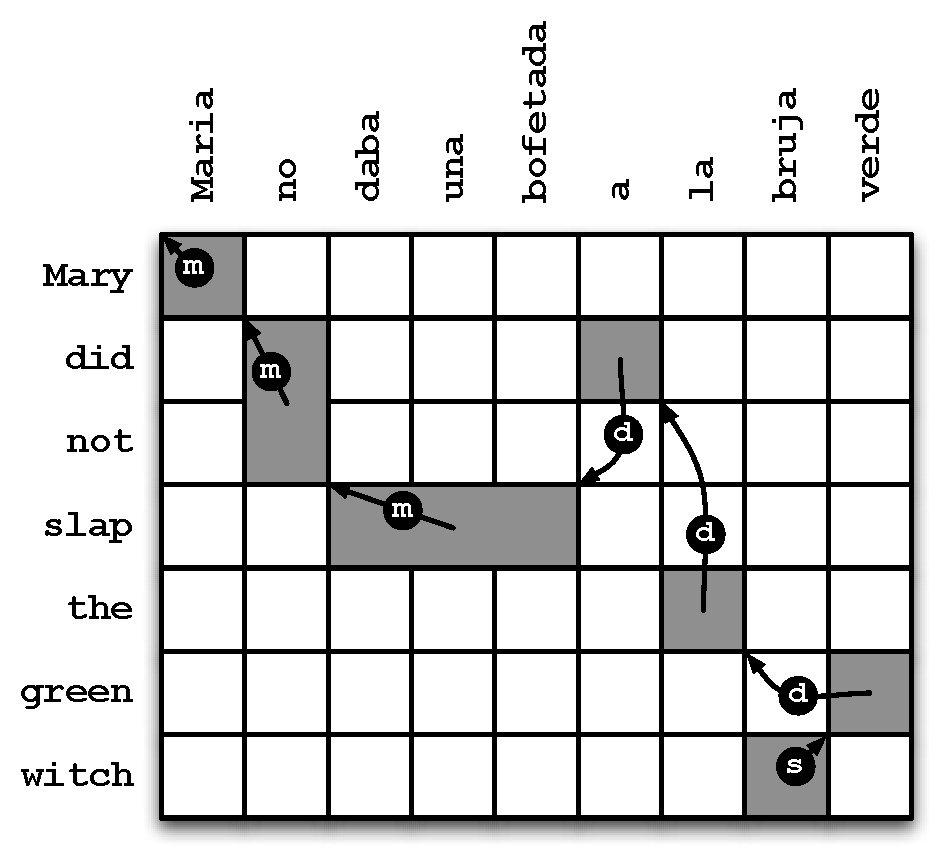
\includegraphics[width=\linewidth]{../figures/reorderfeats/reorderfeats.pdf}
\caption{Example alignment along with three kinds of orientations: monotone (m), swap (s), and discontinuous (d). }
\label{fig:reorderfeats} 
\end{center}
%\vskip -0.2in
\end{figure}\mtodo{\figref{fig:reorderfeats}: switch rows and columns to be consistent with \figref{fig:monoreord}?}

In this work, we will use the same general mathematical formulation, but propose alternative features derived directly from monolingual data.

 \subsection{Lexicon Induction} \label{sect:bckg:lexind}
 
Let us now briefly review relevant prior work on lexicon induction.  In \secref{sect:mono} we will build on this this work specifically to propose alternatives to some of the types of features we outlined in \secref{sect:bckg:smt}.

\todo{Alex: Fill in.}

Most of the previous work evaluates results on a small set of hand selected words (e.g. 100 nouns in \cite{Rapp:1995}).  However, if the objective is to induce large translation tables, as it is in our work, the reported results can be misleading. \mtodo{Diss prev work, but make sure that it comes across that these features are informative.}
 
% ------------------------------------------------

\section{Monolingual Parameter Estimation} \label{sect:mono}

\subsection{Extracting a phrase table without a parallel corpus}  \label{sect:extract}
We propose two competing methods for composing a table of phrase translations without using an aligned parallel corpus. In the first, we extend past efforts in bilingual lexicon induction from monolingual corpora to the induction of multi-word phrases. In the second, we compose a table of phrase pair translations from a bilingual dictionary.

{\it Phrase table induction} Extending work in bilingual lexicon induction to the induction of multi-word translation phrase pairs greatly increases computational cost. Since each source-target pair must be scored, the induction requires $n^2$ comparisons.  The models must  compute $|V_{s}| * |V_{t}|$ similarity scores, where $|V_{s}|$ and $|V_{s}|$ are the number of unique items in the source and target vocabularies. When we search for phrase pairs instead of word pairs, $|V|$ increases to the number of unique {\it n}-grams. Exhaustively scoring all phrase pairs up to length three requires computing scores between the set of unique unigrams, bigrams and trigrams in the source and target languages.  Although we can limit the source phrases that we consider to those that appear in a given test set, we must still compare them to all target phrases.  Because this search space is very large, we aggressively prune it.   Specifically, 
we compare phrases in the same frequency bands \cite{Uszkoreit:2010}, require that each phrase-pair contain at least one word-pair from our seed bilingual dictionary, and prune all very low frequency target phrases. %\todo{Alt wording:} We compare  each source side phrase only to target side phrases that occur in the same frequency band (according to the frequencies in two monolingual corpora). Of those target side phrases, we keep only the ones with at least one \mtodo{discuss dictionary parameters} word translating into a word in the source side phrase. 

To determine whether our pruning parameters were reasonable, we evaluated what percent of the items from a bilingually induced phrase table were retained.  Rather than consider all items from the phrase table (since many of them are bad), we considered only those phrase-pairs that were used by the decoder when translating a test set.\footnote{To determine which phrase pairs were used by the decoder, we used Moses decoder's trace function to find the set of phrases used in decoding our test set} We compare our filtered phrase tables to this set of phrase translation rules and attempt to maintain as many of them as possible, while pruning the set of phrase pairs down to manageable size. 

{\it Dictionary-composed phrase table} \mtodo{Chris had a citation for this method}. We compose the table by enumerating all combinations of all translations of each word in a given source side phrase and then producing all word order permutations. Our available \mtodo{citation from this? it's a combination of some of David's dictionaries, I think} Spanish--English dictionary has over 300,000 entries and the resulting phrase table has a large amount of overlap with the decoder table, as shown in Table \ref{table:prune}. However, low-resource languages, dictionaries, in the cases that they even exist, are not as complete. We expect the performance of our dictionary-composed phrase table to be the upper bound for the performance of an induced-dictionary-composed table for truly low-resource languages. 

%Our baseline phrase table is generated using a bilingual dictionary. For each Urdu test set phrase up to length three, we generated English phrases from all combinations of dictionary translations and all possible reorderings. For the baseline and our pruning methods, the number of filtered phrase pairs and the percent of phrases used by the Moses decoder not pruned away are given in Table \ref{table:prune}.  

\begin{table}
\small
\begin{center}
\label{table:prune}
\begin{tabular}{|c|c|c|c|c|}
\hline
Pruning 	& Phrase	& Search & 	Findable 	& Findable \\
filters	& Pairs	&  Space & Types 	&  Tokens \\
\hline
Unpruned & 1.6 T & 100\% & 100\% & 100\% \\
Dict permut. & 74 M & $<$.01\% & X\% & X\% \\
Frequency &  31 B & 2\% & 75\% & 81\% \\
Freq + Dict & 566 M & $<$.04\% & 42\% & 50\% \\
\hline
\end{tabular}
\caption{This shows the tradeoff between pruning the phrase pair search space and the accuracy of the final set of phrase pairs. The findable types and tokens measures refer to the percent of phrase types and tokens used by Moses to decode a test set that are not pruned away. }\label{pruning-phrase-comparisons}
\end{center}
\end{table}


%Second round of pruning: after monolingual feature extraction, before re-ordering estimation. \todo{Needs to be discussed after explanation of those methods?}

\subsection{Phrase scoring} \label{sect:score}

In place of phrase scores estimated from bilingual alignments, we propose similarity scores computed (almost) solely from monolingual resources.  In this section, we introduce two kinds of scores we call {\em phrasal} and {\em lexical similarity} features.  The former score the entire phrases, while the latter use alignments across phrases pairs, if available, to score at the lexical level.  The motivation is similar to the two kinds of features we introduced in \secref{sect:bckg}: lexical similarity features are informative for rare phrases with less reliable phrasal similarity scores.

\subsubsection{Phrasal similarity features} \label{sect:phrasalfeats}

\begin{figure}
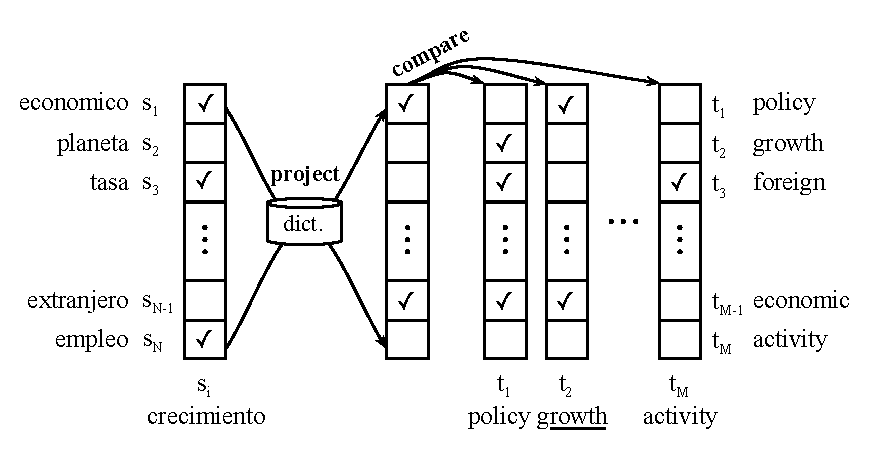
\includegraphics[width=\linewidth]{../figures/contextual/contextual}
\caption{Scoring contextual similarity: first, contextual vectors are projected using a small seed dictionary and then compared with the target language candidates.}
\label{fig:contextual}
\end{figure}

\noindent\emph{Contextual similarity.}  We extend the vector space approach of \cite{Rapp:1999} to compute similarity between \emph{phrases} in source and target language.  More formally, assume that $(f_{1}, f_{2}, \dots f_{N})$ and $(e_{1}, e_{2}, \dots e_{M})$ are (arbitrarily indexed) source and target vocabularies, respectively (see \figref{fig:contextual}).  A source phrase $f$ (target phrase $e$) is represented with an $N$ ($M$) dimensional vector.  Only the components corresponding to words that appear in the context of $f$ ($e$) in data take on non-zero values, which typically measure how ``unique'' a word is to the context in the dataset.  Next, $f$'s contextual vector is projected by mapping each component to a component in the target space corresponding to its translation (taken from a small seed dictionary), but retaining the source component value.  Finally, the pair ($f, e$) is scored by computing similarity between the (projected) source and target vectors.  Various means of computing the component values and vector similarity measures have been proposed in literature (e.g. \cite{Rapp:1999,Fung:1998}).  While the quality of the resulting induced lexicon depends on the data, we found the following to work best in our experiments.  We compute the value of the $k$-th component of $f$'s contextual vector  as follows: 

\begin{equation*}
w_{k}^{(i)} = n_{i,k} \times (log( {n / n_{i}}) + 1)
\end{equation*}

\noindent where $n_{i,k}$ and $f_{k}$ are the number of times $f_{k}$ appears in the context of $f_{i}$ and in the entire corpus, and $n$ is the maximum number of occurrences of any word in the data.  Intuitively, the more frequently $f_{k}$ appears with $f_{i}$ and the less common it is in the corpus in general, the higher its component value.  Similarity between two resulting vectors is measured as a cosine of the angle between them.\\

\begin{figure}[t]
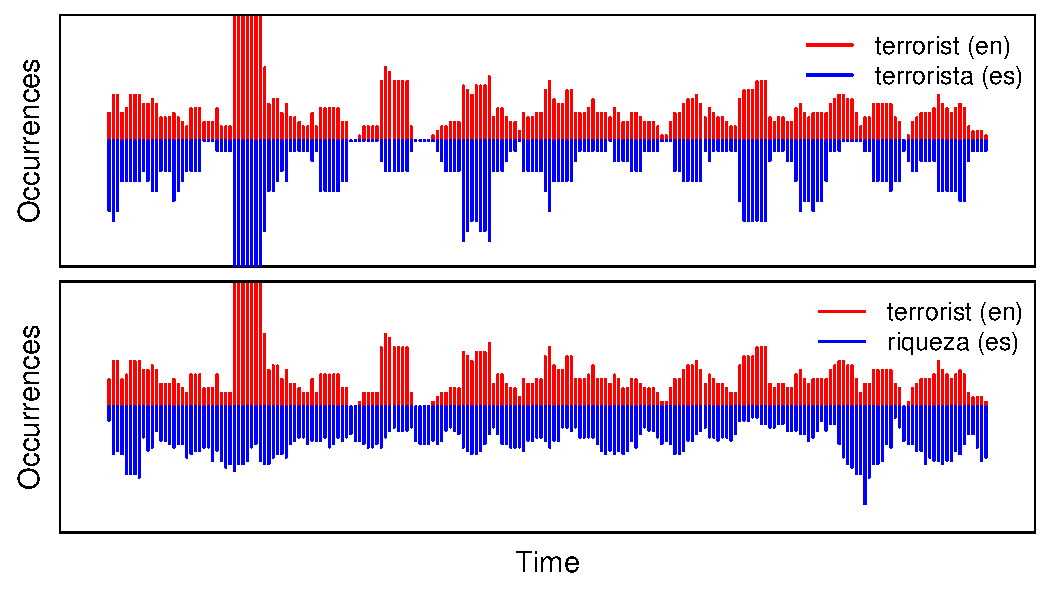
\includegraphics[width= \linewidth]{../figures/temporal/temporal}
\caption{Temporal histograms of the English word {\em terrorist}, its Spanish translation {\em terrorista}, and the words {\em ataques}  (attacks) and {\em riqueza} (wealth) collected from a subset of the Europarl corpus. While the correct translation has a better temporal match, the word {\em ataques} is often used around the same dates and shares a number of peaks of occurrences with the word {\em terrorist}.  The third word has a distinctly different temporal signature.}
\label{fig:temporal}
\end{figure}

\noindent\emph{Temporal similarity.} Online content is often published along with temporal information: news feeds, for example, are comprised of news stories annotated with date and time of publication.  The feeds are specialized for the target geographical locations and vary in content across languages.  Still, many events are deemed relevant to multiple audiences and the news stories related to them appear in several languages, although rarely as direct translations of one another.  Phrases associated with these events will appear with increased frequency in multiple languages around the dates when these events are reported (see \figref{fig:temporal}).  Such weak synchronicity provides a cue about the relatedness of phrases across the two languages.  In order to score a pair of phrases across languages, we can compute the similarity of their temporal signatures. To generate a time sequence for a given word, we first sort the set of (time-stamped) documents of our corpus into a sequence of equally sized temporal bins.  We then count the number of occurrences of a phrase in each bin.  Changing the size of the bin or computing counts in a sliding window instead can recover some accuracy if the temporal alignment between two languages in our dataset is poor \cite{Klementiev:2006b}.  Finally, we normalize the sequence and use the cosine measure to score similarity. 

\subsubsection{Lexical similarity features}  \label{sect:lexfeats}

\noindent\emph{Contextual and Temporal similarity.}  If word alignments within a phrase pair are available, we can use them to compute a lexical similarity score for the pair.  We first compute an average similarity score (contextual or temporal) over all aligned words across the two phrases.  We then scale the score by the proportion of aligned words in the two phrases, effectively penalizing poorly aligned phrase pairs.\mtodo{Mention that it is the average of both forward and backward alignments?}\\

\noindent\emph{Orthographic / phonetic similarity.} Etymologically related words often retain similar spelling across languages with the same writing system, and the edit distance can be used to measure their similarity.  We use word alignments as before to score entire phrases for orthographic similarity.\mtodo{Not done quite the same as above but will glance over it.} We can also extend this idea to language pairs not sharing the same writing system, since many cognates and transliterated words remain phonetically similar.  Transliterations can be generated for tokens in a source phrase (e.g. \cite{Virga:2003,Irvine:2010a}), with phrase similarity computed as before.\\

In our experiments in \secref{sect:exp}, we will focus on the phrase scores introduced in this section.  However, note that various other similarity scores can be computed depending on the available monolingual data (and its associated metadata), (see, e.g. \cite{Schafer:2002}).

\subsection{Reordering} \label{sect:order}

\begin{figure}[t]
%\vskip 0.1in
\begin{center}
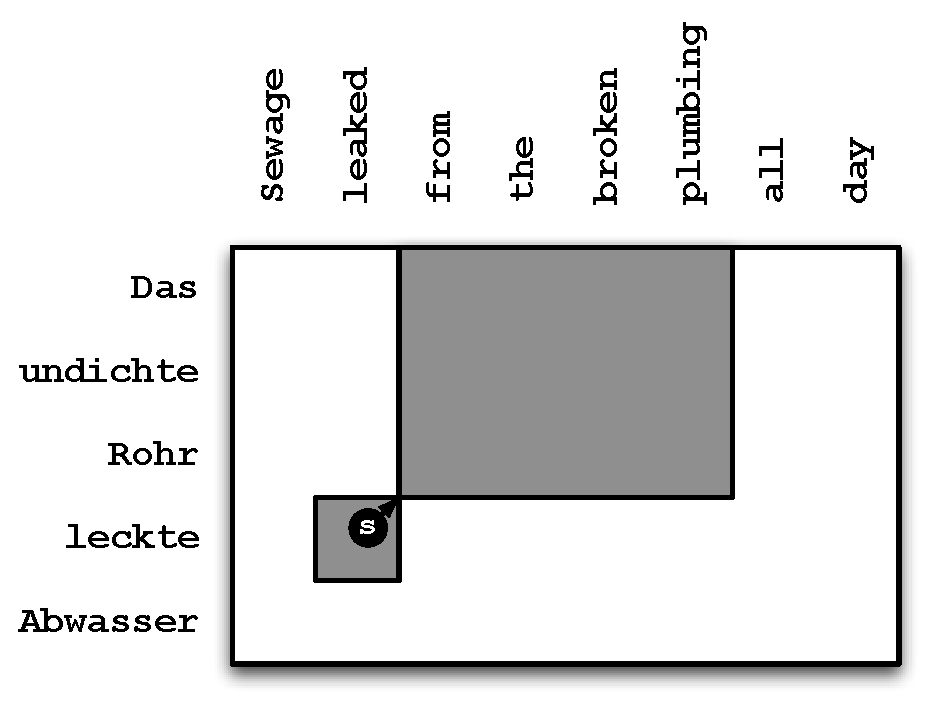
\includegraphics[width=\linewidth]{../figures/monoreord/monoreord.pdf}
\caption{Collecting phrase ordering statistics for a de-en phrase pair (\emq{leckte}, \emq{leaked}).  The longest preceding phrase \emq{Das undichte Rohr} in source, has a phrase table translation \emq{from the broken plumbing} appearing after the target phrase.}
\label{fig:monoreord}
\end{center}
\vskip -0.2in
\end{figure}

In the phrase-based SMT pipeline we reviewed in \secref{sect:bckg:smt}, phrase pair orientation statistics were collected from induced word alignments.  We keep a similar lexicalized reordering model formulation, but infer its parameters from monolingual data instead.  The orientation information for a phrase pair is collected from source and target sentences containing the two phrases as well as other hypothesized translation pairs.  Given a phrase pair ($f$, $e$), the idea is to estimate the probability that other phrases preceding $f$ will precede, follow, or become discontinuous with $e$ in target sentences when translated.  Contextual phrases used to estimate these orientation features for ($f$, $e$) will be all entries in the phrase table.  Consider a simple example on \figref{fig:monoreord}: the phrase pair is ($f =$ \emq{leckte}, $e =$ \emq{leaked}), and a given pair of unaligned sentences also contains a phrase table entry ($f_{b} =$ \emq{Das undichte Rohr}, \emq{from the broken plumbing}).  In this example, the phrase $f_{b}$ preceding $f$ in the source sentence swaps order with $e$ in the target.  When collected a over large unaligned bilingual corpora, we expect the swap, monotone, and discontinuous counts to provide good estimates for the orientation features.  Note that multiple phrases may immediately precede $f$ and appear in the phrase table; however, we only use the longest of them to collect reordering counts.\mtodo{Explain why?}

The algorithm on \figref{fig:algoreorder} estimates monotone, swap, and discontinuous orientation features $(p_m, p_s, p_d)$ for a phrase pair ($f, e$).  It begins by calling {\tt \small CollectOccurs()} to collect the longest phrase table phrases ($B_f$) preceding $f$ in source monolingual data, as well as preceding ($B_e$), following ($A_e$), and discontinuous ($D_e$) phrases with $e$ in the target language data.  For each uniques phrase $f_{b}$ preceding $f$, translations are then looked up in the phrase table $\emph{T}$.  Next, we count\footnote{$\#_{L}(x)$ returns the count of object x in list L.} how many translations $e^*$ of $f_b$ appeared before, after or were discontinuous with $e$ in the target language data.  Finally, the counts are normalized and returned. \mtodo{Be more specific about the out-of-order counts?}  The algorithm requires a single pass through the data to collect contextual phrases for the entire phrase table and its running time is quadratic in the size table.\mtodo{Check}

\SetAlFnt{\relsize{-1.5}}

\begin{algorithm}[t]

 \SetKwFunction{CollectOccurs}{CollectOccurs}
 \SetKwBlock{Body}{}{}
 \SetCommentSty{text}
 \SetFuncSty{text}

 \hrule \vskip 0.2cm

  \KwIn{Source and target phrases $f$ and $e$,\\
  \hskip 0.85cm Source and target monolingual corpora $\emph{C}_f$ and $\emph{C}_e$,\\
  \hskip 0.85cm Phrase table pairs $\emph{T} = \{(f^{(i)}, e^{(i)})\}_{i=1}^{N}$.}
  \KwOut{Orientation features ($p_m, p_s, p_d$).}
  
  \vskip 0.2cm \hrule \vskip 0.2cm

  $S_f \leftarrow$ sentences containing $f$ in $\emph{C}_f$\;
  $S_e \leftarrow$ sentences containing $e$ in $\emph{C}_e$\;
  
  $(B_f, -, -) \leftarrow \CollectOccurs(f, \cup_{i=1}^{N} f^{(i)}, S_f)$\;
  $(B_e, A_e, D_e) \leftarrow \CollectOccurs(e, \cup_{i=1}^{N} e^{(i)}, S_e)$\;
    
  $c_m = c_s = c_d = 0$\;
  
  \vskip 0.1cm 

  \ForEach{uniques $f_b$ in $B_f$} {
    \ForEach{translation $e^{*}$ of $f_b$ in $\emph{T}$} {

      $c_m = c_m + \#_{B_e}(e^{*})$\; 
       $c_s = c_s + \#_{A_e}(e^{*})$\; 
       $c_d = c_d + \#_{D_e}(e^{*})$\; 
    }
  }
  
  $c \leftarrow c_m + c_s + c_d$;
    
  \Return{$({c_m \over c}, {c_s \over c}, {c_d \over c})$}

  \vskip 0.2cm \hrule \vskip 0.2cm

  \CollectOccurs{$r$, $R$, $S$} \Body{
   $B \leftarrow ()$; $A \leftarrow ()$; $D \leftarrow ()$\;

    \ForEach{sentence $s \in S$} {
      \ForEach{occurrence of phrase $r$ in $s$} {
        $B \leftarrow B$ + $($longest preceding and in $R)$\;
        $A \leftarrow A$ + $($longest following and in $R)$\;
        $D \leftarrow D$ + $($longest discontinuous and in $R)$\;
      }
    }
    
    \Return{($B$, $A$, $D$)}\;
  }
  
  \vskip 0.2cm \hrule \vskip 0.2cm

  \caption{Estimating reordering probabilities from monolingual data.} \label{fig:algoreorder}
  %\vskip -0.2in
\end{algorithm}

% ------------------------------------------------

\section{Experiments} \label{sect:exp}

We use the Spanish-English\mtodo{Add German if done in time.} subset of the Europarl version 5 corpus \cite{Koehn:2005} in all of the experiments below.  However, we treat the two sides of the corpus as two independent {\em monolingual} corpora.  We use the Moses SMT toolkit\mtodo{Add a moses citation} and a language model trained on the English side of Europarl.  With the exception of maximum phrase length (set to 3 in our experiments\mtodo{Add our curve?}), default values were used for all of the parameters.
\todo{A brief outline of the experiments}

\subsection{Bilingual lexicon induction for SMT}

\begin{figure}[t]
%\vskip 0.1in
\begin{center}
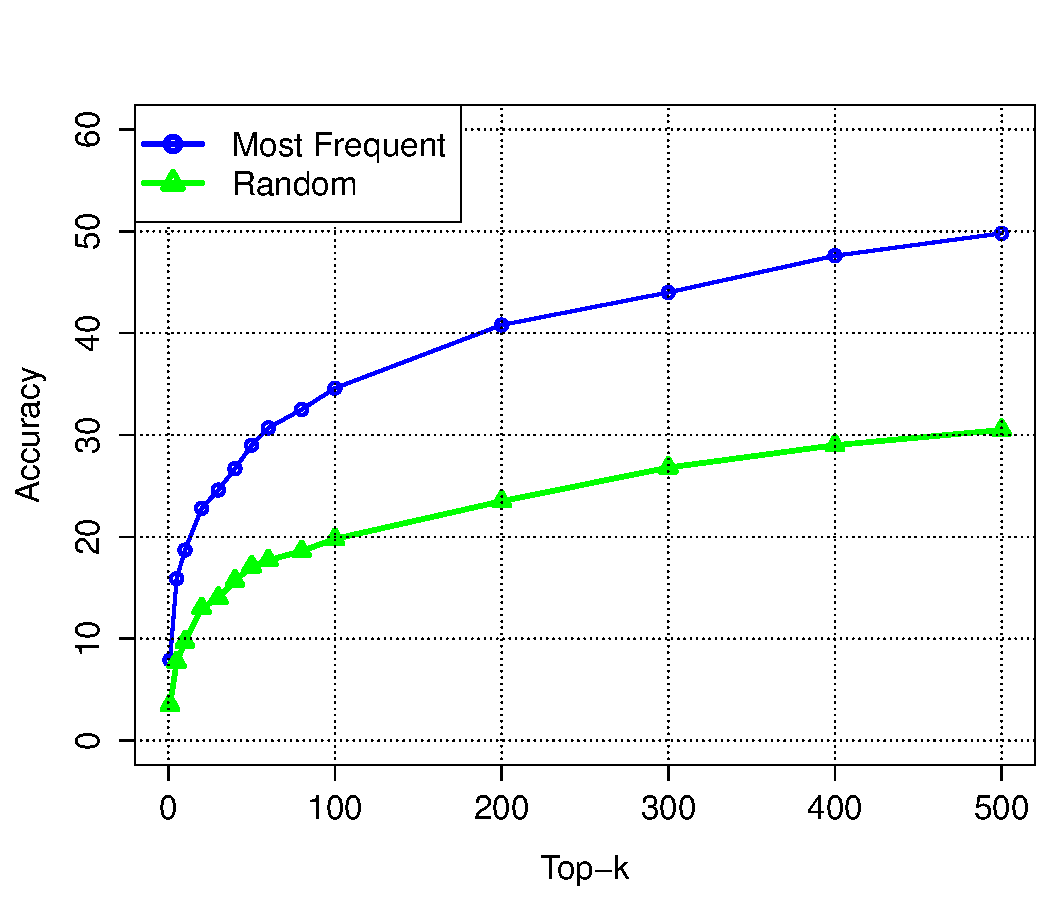
\includegraphics[width=\linewidth]{../figures/lexinduct/lexinduct.pdf}
\caption{Accuracy on wikipedia for most frequent and random 1000 source words. }
\label{fig:lexinduct}
\end{center}
\vskip -0.2in
\end{figure}

\subsection{Feature lesions}

We begin with a series of experiments where we remove individual features in order to get a sense of the relative contribution to the overall system performance on the English-Spanish language pair. Four rightmost bars on \figref{fig:lesion} summarize the results.  When both phrase and orientation features are derived from word alignments ({\bf A.A}, the standard features functions defined in \secref{sect:bckg:smt}), the system reaches 21.87 BLEU.  Next we replace orientation features with random values ({\bf A.R}) and drop phrase table features ({\bf --.A}).  While phrase table features account for a substantial performance difference (9 BLEU points), dropping orientation features affects the system score relatively little.  This is not surprising, since the word order is generally preserved in Spanish to English translations.  Finally, both dropping phrase scores and replacing orientation features with random values ({\bf --.R}) results in 5.5 BLEU. \mtodo{Drop A+PL.A, move to next section}

\begin{figure}[t]
%\vskip 0.1in
\begin{center}
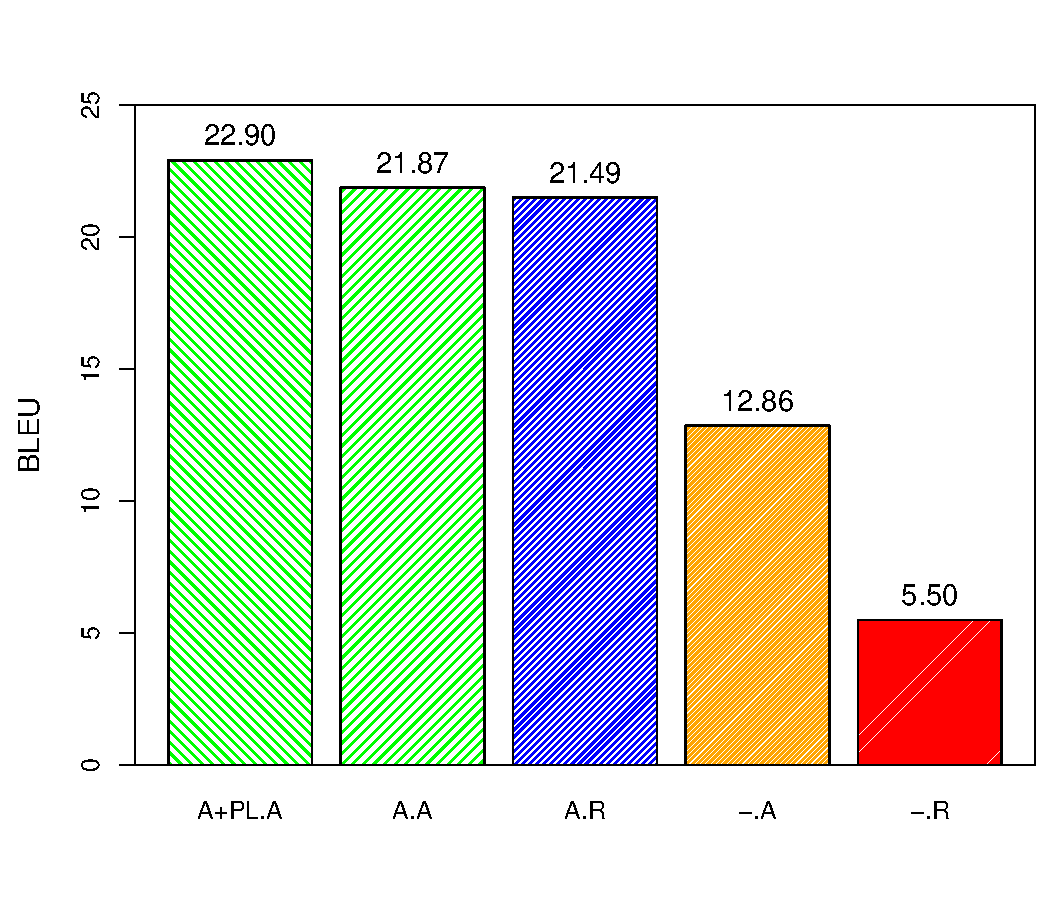
\includegraphics[width=\linewidth]{../figures/lesion/lesions.pdf}
\caption{Contributions of individual features to overall system performance: both phrase and orientation features derived from word alignments ({\bf A.A}), orientation features replaced with random values ({\bf A.R}), dropped phrase features ({\bf --.A}), and dropped phrase features and random orientations ({\bf --.R}).  Adding monolingual features improves performance: phrase scores are augmented with phrasal and lexical monolingual similarity scores ({\bf A+PL.A}).}
\label{fig:lesion}
\end{center}
\vskip -0.2in
\end{figure}

Next, we replace the feature functions with their monolingual equivalents.

\subsection{Monolingual features}




%\subsection{Single language}

%\begin{enumerate}
%\item {\em Phrase features}.  (a) Augment phrase scores with mono features.  If we see better performance, reduce the amount of parallel data until it matches the performance of the original system.  Make the tradeoff argument.  (b) ({\bf lesion experiments}) See how well we do with mono features alone.
%\item {\em Orientation features}. Use mono orientation features.
%\item {\em Induce phrase table}.
%\item {\em Put everything together}.  Run the entire pipeline.
%\end{enumerate}

%\subsection{Big experiment}

%Now, run the entire pipeline on a handful of languages extracting monolingual features from the Gigaword and our crawls.

% ------------------------------------------------

\section{Discussion} \label{sect:disc}

% ------------------------------------------------

\section{Conclusions and Future Work} \label{sect:conc}

First to make use of plentiful monolingual data to reduce the dependence on expensive parallel data.  In particular:

\begin{itemize}
\item We plan to run this on real data for low resource languages.  We are have been actively collecting newswire data, which we plan to make available to the community.
\item Language pairs with different writing system: use transliteration for edit distance features (as suggested in \secref{sect:phrasalfeats}).
\item Showed that augmenting standard pipeline with monolingual features helps.
\item Demonstrated that monolingual features are informative enough on their own for a competitive system.
\item Proposed an algorithm for estimating orientation probabilities from monolingual data alone.
\item Build complete systems for X low-resource languages.
\end{itemize}

%\section*{Acknowledgments}
%The authors would like each other and their parents.

\bibliographystyle{acl}
% you bib file should really go here 
\bibliography{lowresmt}

\end{document}
